%%
%%

\documentclass[twocolumn, nofootinbib, secnumarabic, amssymb, nobibnotes, aps, prd]{revtex4-2}
\usepackage{graphicx}
\usepackage{multirow}
\usepackage[table,xcdraw]{xcolor}
\usepackage{subfigure}
\usepackage{amsmath}
\usepackage{afterpage}
\usepackage{placeins}

\newcommand{\revtex}{REV\TeX\ }
\newcommand{\classoption}[1]{\texttt{#1}}
\newcommand{\macro}[1]{\texttt{\textbackslash#1}}
\newcommand{\m}[1]{\macro{#1}}
\newcommand{\env}[1]{\texttt{#1}}
\setlength{\textheight}{9.5in}

\begin{document}

%show just eight optimized models w/o error
%comparison of base model, then cleaned - extra trees
%ADD THIS REF: https://doi.org/10.1515/znb-2019-0103

\begin{abstract}
One of the long-standing challenges in the last century is to find near room-temperature superconductors. There are limited technological applications due to the insufficient fundamental understanding of the physics of these unconventional superconductors. Researchers have recently explored machine learning models to predict superconducting critical temperatures in several papers, but these researchers have not attempted to quantify uncertainty. This paper expands upon that work by exploring alternative models to improve the utility of such models and addressing the  uncertainty quantification. Our research produced multiple models exceeding R2 scores of 0.9 and mean absolute errors below 4.5K. We also made our code available publicly on Github and intend for it to be as functional and reusable as possible. 
\end{abstract}

\keywords{superconductors; machine learning; regression; critical temperatures; matminer} %add "showkeys" to document class to add keywords to document

\title{Predicting Superconducting Critical Temperatures with Uncertainty Quantification using Supervised Machine Learning}

\author{K. Kleinasser, Cornell University, Ithaca, NY}
\altaffiliation{Lycoming College, Williamsport, PA}
\email{klekirk@lycoming.edu}

\maketitle
%\tableofcontents

\section{Introduction}
%get rid of subsections, bulletpoint types of models, incl. references
%model discussions after dataset
Superconductors are materials that lose all electrical resistance at low temperatures. These materials have a critical temperature ($T_C$) at which they lose their resistance. Most have very low critical temperatures, but “unconventional superconductors” can have critical temperatures as high as room temperature under non-atmospheric conditions. 

Electrons in superconductors form Cooper Pairs below their critical temperature. These pairs of electrons are held together with phonouns, which are atomic-level collective excitations. Phonouns are similar to photons in that they also have particle-like properties \cite{rohlf_1994, BussmannHolderKeller2020}.

Unconventional superconductors are still not well understood and remain an open question in Physics. Understanding them could lead to the discovery of superconducting materials stable at room temperature under atmospheric conditions. Such a material would have large implications, such as super efficient electricity transfer and vast efficiency improvements for applications like particle accelerators and power lines.

Machine learning can be an excellent asset in the search for such superconducting materials. An accurate model that can predict critical temperature based on composition attributes could be used to vet candidate materials before experimental testing, allowing experimentalists to focus on promising materials. 

Calculating uncertainty is also important, as it can give research a confidence range for a machine learning model's prediction. This paper attempts to create an accurate model with uncertainty quantification, allowing experimentalists to predict critical temperatures with the confidence intervals.

\section{Methodology}
\subsection{Database}
We chose to use data sourced from one most popular experimental datasets, the supercon database from Japan's National Institute for Materials Science. This dataset is not available publicaly from the National Institute for Materials Science's website, so we used data obtained from \cite{Stanev2018}. This is the same database, but Stanev Et al. resolved conflicts in the data and dropped obvious erroneous data.

This datasets contains 16,414 superconductor chemical compositions and their experimentally measured critical temperatures. According to \cite{Stanev2018}, around 5700 of these materials are cuprates and 1500 are iron-based. More demographic metadata is available in their paper. 

We dropped materials that did not have a critical temperature recorded, about 4,000 materials. This leaves us with a dataset of around 12,500 materials. %IMPORTANT - cite Hamidieh if we use the other dataset

\begin{figure}[!h]
   \centering % add numbers to columns
   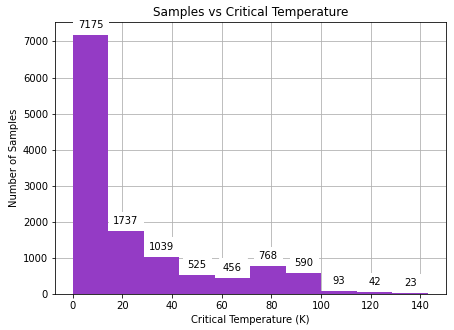
\includegraphics[width=\columnwidth]{images/dataset_histogram.png}
   \caption{A histogram of critical temperatures in the dataset. Most superconductors are found at low temperatures and this dataset is representative of that.} %more info in caption
\end{figure}\label{fig:data-histogram}

In the remaining data, there are 6,188 samples with a critical temperature below 10K and 6,210 samples above 10K. There are 159 samples with temperatures above 100K and 0 samples above 145K. A histogram represents this information graphically in Figure~\ref{fig:data-histogram}. Since most of this data is at low temperatures, we can expect less accuracy in our models for higher critical temperature superconductors.

Most superconductor databases do not include enough information to train an effective machine learning model, but such data can be extracted from the data they do provide. We use matminer to produce our features from the provided material data. Matminer is a python library that generates data from various measured properties of a material \cite{WARD201860}. Matminer collects existing calculations into a machine learning friendly python package. %Our matminer workflow is shown in Figure~\ref{fig:matminer-flowchart}.

% \begin{figure}[!htb]
%    \centering
%    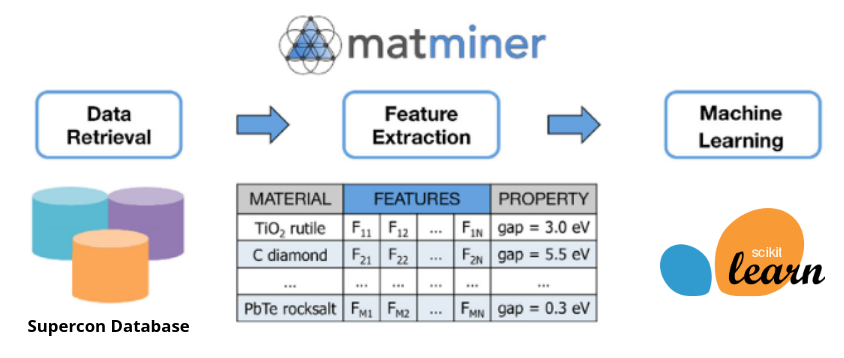
\includegraphics[scale=0.25]{flowchart.png}
%    \caption{Flowchart illustrating our matminer usage, modified from official matminer graphic \cite{WARD201860}.}
% \end{figure}\label{fig:matminer-flowchart}

Our database only provides the superconductor composition data. Matminer's featurizers can generate 53 features from the composition of a material. If we had band structure or other data, we could produce more information that we could use in our model.

\subsection{Machine Learning}

Previous papers have used random forest models to predict critical temperature [citation needed], but this paper will examine eight models before settling on two for further investigation. All models are implemented with Scikit-Learn, with the notable exception of a mlens superlearner \cite{scikit-learn, flennerhag:2017mlens}. We will also use MAPIE models for uncertainty, discussed in Section~\ref{sec:uncertainty}.

We decided to test a variety of machine learning models to ensure we would find an optimal model. These models are listed below:

\begin{itemize}
  \item Linear Regression
  \item Support Vector Regression (SVR)
  \begin{itemize}
  		\item  SVR makes predictions with decision boundaries, which are lines parallel to the regression line or curve. The model aims to maximize the amount of data within the decision boundaries and has hyperparameters to modify sensitivity to prevent overfitting.\footnote{Overfitting occurs when a model is trained to be too specific to a particular dataset and is not generalizable.}
  \end{itemize}
  \item Elastic Net
  \begin{itemize}
  		\item Elastic Net uses L1 and L2 penalties to stabilize a linear model.
  \end{itemize}
  \item Bayesian Ridge
  \begin{itemize}
  		\item Bayesian Ridge uses probability distributors instead of point estimates for a linear model.
  \end{itemize}
  \item Decision Tree
  \begin{itemize}
  		\item Decision trees are very interpretable - they break predictions into nodes of the tree, eventually leading to a prediction value. These trees can be represented graphically and show how they produce results, unlike most machine learning models.
  \end{itemize}
  \item KNeighbors (KNN)
  \begin{itemize}
  		\item KNN models are a little different, they store all the data and predict values based on a similarity measure. The model looks at a specified number of similar neighbors to produce a prediction.
  \end{itemize}
  \item Random Forest Regression (RFR)
  \begin{itemize}
  		\item RFR is an ensemble method that uses numerous decision trees and subsamples the data with replacement. This means that the model replace data after using it in a subset.
  \end{itemize}
  \item Extra Trees
  \begin{itemize}
  		\item Extra Trees is like RFR, but it does not replace the data after use in a subset.
  \end{itemize}
  \item Superlearner
  \begin{itemize}
  		\item Our superlearner is a mlens model that can combine multiple high-scoring Scikit-Learn model predictions and sometimes improve the performance from the individual models.
  \end{itemize}
\end{itemize}\label{itm:models}

%We started our model search with some linear models. Besides the base Linear Regression model, we used linear (and polynomial) Support Vector Regression (SVR) models. We also trialed Elastic Net and Bayesian Ridge models. , and Bayesian Ridge uses probability distributors instead of point estimates.

%Additionally, we trialed Decision Tree and KNeighbors (KNN) models. Decision trees are very interpretable - they break predictions into nodes of the tree, eventually leading to a prediction value. These trees can be represented graphically and show how they produce results, unlike most machine learning models. KNN models are a little different, they store all the data and predict values based on a similarity measure. The model looks at a specified number of similar neighbors to produce a prediction.

%Finally, we tried multiple ensemble models - Random Forest Regression (RFR), Extra Trees, and a superlearner. RFR models use numerous decision trees and subsamples the data with replacement. This means that the model replace data after using it in a subset. Extra Trees is like RFR, but it does not replace the data after use in a subset. The final ensemble model we tested is a superlearner, a model that can combine multiple high-scoring Scikit-Learn model predictions and sometimes improve the performance from the individual models.

\subsection{Quantifying Uncertainty}\label{sec:uncertainty}
Our evaluation functions can produce uncertainty calculations using forestci, mapie, or lolopy \cite{Polimis2017, Taquet2022, Hutchinson2022}. 

Forestci is python implementation of an algorithm from \cite{Wager2014} that predicts confidence intervals for random forest models. It is the fastest of the uncertainty methods listed. 

The Model Agnostic Prediction Interval Estimator (MAPIE) python library is more recent implementation of jackknife based on \cite{Foygel2020}. MAPIE uses various resampling methods. Most methods require the use of MAPIE's own MapieRegressor, which accepts an Scikit-Learn regressor and keeps track of uncertainty as the model is trained. We chose to use the MAPIE-plus method, which is based of the Jackknife+ algorithm. This is the default uncertainty method for MAPIE and is recommended by the developers.

MAPIE also has a prefit method, but it is difficult to extract uncertainty bars for individual points from this data - it splits a celebration set off the test set to generate uncertainty, so it can't be easily added to our plot of test set predictions. Thus, we will only compare the normal MAPIE methods with the other libraries. MAPIE trains much slower than other models, particularly on our superlearner, but it is still considerably faster than our final uncertainty model, lolopy.

Lolo is a Scala random forest machine learning library and is not a native python implementation. Lolopy is a python wrapper for lolo, but this implementation is very slow for large datasets. We were unable to successfully train a lolopy model due to these factors and time limitations of the project, but our code supports lolopy models.

\subsection{Project Structure} %MENTION PANDAS/NUMPY/ETC
The source code used for this paper is available publicly on github at \url{https://github.com/sylphrena0/classe2022}. This repository also includes the source files for this latex paper, data files, images, and documentation files.

Our research uses numpy and pandas throughout our code to handle arrays and tabular data \cite{Harris2020array, Reback2020pandas}. We also use matplotlib and seaborns to generate our graphs \cite{Hunter2007, Waskom2021}.

The code is split into multiple python files so processes could be completed in stages and to maintain readability in the code. Most of our testing and final training was completed in juypter notebooks, but some computations were highly computationally expensive and needed to be run remotely. For these jobs, we created simple python files and made bash scripts to run them on Cornell's CLASSE compute farm. We also made several bash aliases and functions to simplify the compute farm workflow, which are also available on the github repository. 

Since we used multiple files, we chose to create shared dependencies files where we defined functions to import data, train models, and generate our graphs. These files are then imported in all the relevant scripts to reduce redundancy. More detailed explainations of the purpose of each file is available in the github readme file and documentation within the files.

\subsection{Project Evaluation}

First, the featurizer script imports the dataset, extracts features from the material compositions, and exports the csv data. This script is one of the most computationally expensive and takes several hours to run on the CLASSE compute farm with 64 dedicated cores.

After the features are exported, our analysis jupyter notebook imports the data with the shared import function and exports histograms and a correlation matrix. 

Next, the training\_single jupyter notebook or script can train individual models with the shared evaluation functions. This is used to get a landscape of initial performance before optimization. After training, the function plots the actual $T_C$ versus the model prediction, using a heatmap to visualize the difference from the ideal prediction.

The optimizer script then uses a grid of manually defined hyperparameters to optimize models based on R2 score. This allowed significant improvements to baseline models. After optimization, the optimized models can be plotted in our single training notebook. After confirmation that the model is better than the baseline, the models can then be plotted together in a single graph using our bulk training notebook. 

We evaluated our models using several metrics - R2 scores (R2) for regression evaluation, Mean Squared Error (MSE) and Mean Absolute Error (MAE) for error evaluation, and MAPIE Effective Mean Widths (MWS) for uncertainty evaluation.

\section{Results}
\subsection{Model Optimization}
Each model's hyperparameters\footnote{Hyperparameters are machine learning parameters that change how a model is trained.} were optimized with various optimization methods. Optimization can be computationally expensive, so we chose to optimize on a randomly selected subset of 2,000 materials, using a numpy random state for reproducibility. To start, we used Scikit-Learn's GridSearchCV, which tests combinations from a grid of hyperparameters and returns the best performing model based on a specified metric. 

We also implemented Bayesian optimization using Gaussian Processes methods from the Scikit-Optimize library \cite{head_tim_2021_5565057}. Bayesian optimization attempts to optimize models intelligently, instead of randomly testing specified hyperparameters. We provide a range of hyperparamters values for Bayesian optimization to test, and the algorithm uses acquisition functions to decide which specific values to use within the specified range. This is different from GridSearchCV, which is simpler but can take much longer to find optimal hyperparameters. We only implemented Bayesian optimization on our top models.

\begin{table}[!h]
   \centering
   \resizebox{\columnwidth}{!}{%
   \begin{tabular}{clcccc}
   \hline
   \multicolumn{1}{l}{} & \multicolumn{1}{c}{\textbf{Optimizer}} & \textbf{R2}                   & \textbf{MSE}                    & \textbf{MAE}                  & \textbf{MWS}                   \\ \hline
                        & None                                   & 0.910                         & 71.956                          & 4.360                         & 38.916                         \\
                        & \textbf{GridSearchCv}                  & \cellcolor[HTML]{D9EAD3}0.911 & \cellcolor[HTML]{D9EAD3}71.265  & \cellcolor[HTML]{D9EAD3}4.315 & \cellcolor[HTML]{D9EAD3}38.505 \\
                        & Bayesian – PI                          & 0.911                         & 71.586                          & 4.329                         & 38.061                         \\
                        & Bayesian – EI                          & 0.910                         & 72.136                          & 4.335                         & 38.265                         \\
   \multirow{-5}{*}{\textbf{\rotatebox[origin=c]{90}{\parbox[c]{2cm}{\centering Random Forest}}}}   & Bayesian – gp\_hedge                   & 0.908                         & 73.659                          & 4.399                         & 38.203                         \\ \hline
                        & None                                   & 0.927                         & 58.780                          & 3.787                         & 36.137                         \\
                        & GridSearchCv                           & 0.926                         & 59.181                          & 3.785                         & 35.625                         \\
                        & Bayesian – PI                          & 0.927                         & 58.860                          & 3.778                         & 35.467                         \\
                        & Bayesian – EI                          & 0.927                         & 58.708                          & 3.779                         & 36.205                         \\
   \multirow{-5}{*}{\textbf{\rotatebox[origin=c]{90}{\parbox[c]{2cm}{\centering Extra\\ Trees}}}}   & \textbf{Bayesian – gp\_hedge}          & \cellcolor[HTML]{D9EAD3}0.927 & \cellcolor[HTML]{D9EAD3}58.706  & \cellcolor[HTML]{D9EAD3}3.771 & \cellcolor[HTML]{D9EAD3}35.635 \\ \hline
                        & None                                   & 0.803                         & 157.928                         & 6.897                         & 58.230                         \\
                        & \textbf{GridSearchCv}                  & \cellcolor[HTML]{D9EAD3}0.824 & \cellcolor[HTML]{D9EAD3}141.308 & \cellcolor[HTML]{D9EAD3}6.503 & \cellcolor[HTML]{D9EAD3}54.446 \\
                        & Bayesian – PI                          & 0.807                         & 154.683                         & 6.748                         & 57.802                         \\
                        & Bayesian – EI                          & 0.812                         & 150.997                         & 6.302                         & 60.035                         \\
   \multirow{-5}{*}{\textbf{\rotatebox[origin=c]{90}{\parbox[c]{2cm}{\centering KNN}}}}   & Bayesian – gp\_hedge                   & 0.790                         & 168.329                         & 6.475                         & 65.486                         \\ \hline
   \end{tabular}%
   }
   \caption{Comparison of optimization methods by model.}
\end{table}\label{tab:optimizers}

\begin{figure*}[t] %star makes figure and caption span both columns
   %star enviroment floats are placed on the top of the next page or on dedicated float pages in revtex, no easy way around it
   \centering
   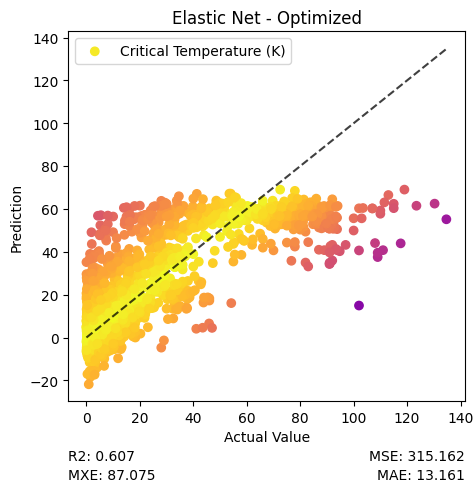
\includegraphics[height=2.25in]{images/subfigures/no_uncertainty/elastic_net_optimized.png}
   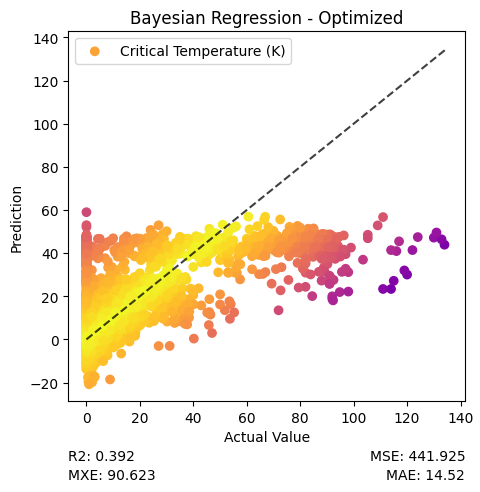
\includegraphics[height=2.25in]{images/subfigures/no_uncertainty/bayesian_regression_optimized.png}
   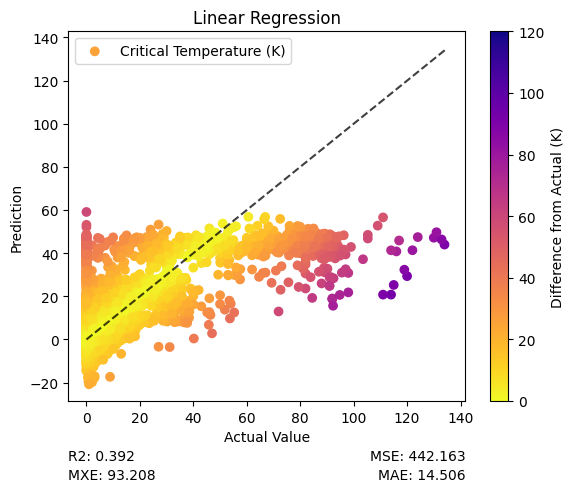
\includegraphics[height=2.25in]{images/subfigures/no_uncertainty/linear_regression.png}
   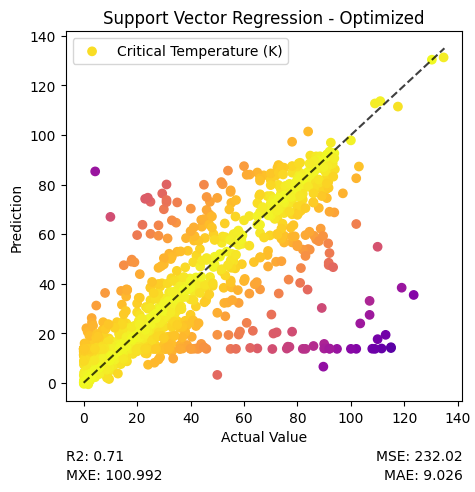
\includegraphics[height=2.25in]{images/subfigures/no_uncertainty/support_vector_regression_optimized.png}
   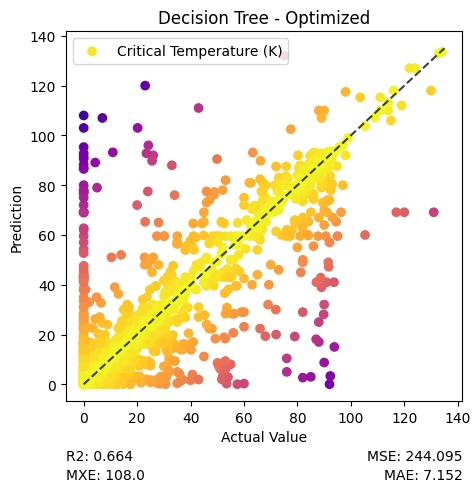
\includegraphics[height=2.25in]{images/subfigures/no_uncertainty/decision_tree_optimized.png}
   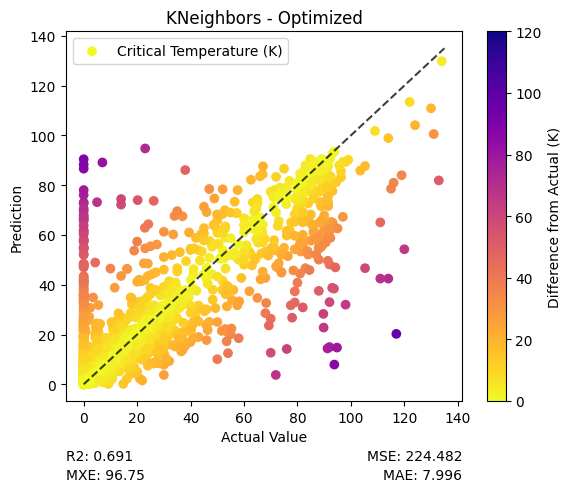
\includegraphics[height=2.25in]{images/subfigures/no_uncertainty/kneighbors_optimized.png}
   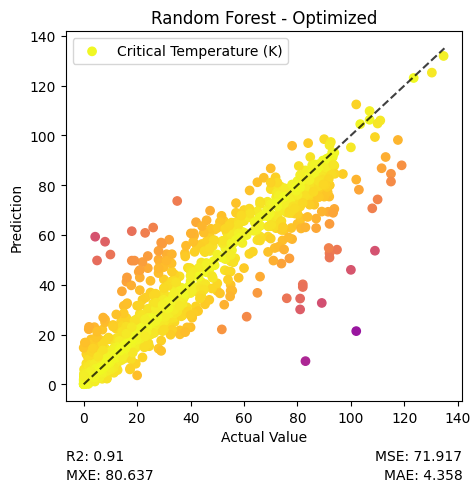
\includegraphics[height=2.25in]{images/subfigures/no_uncertainty/random_forest_optimized.png}
   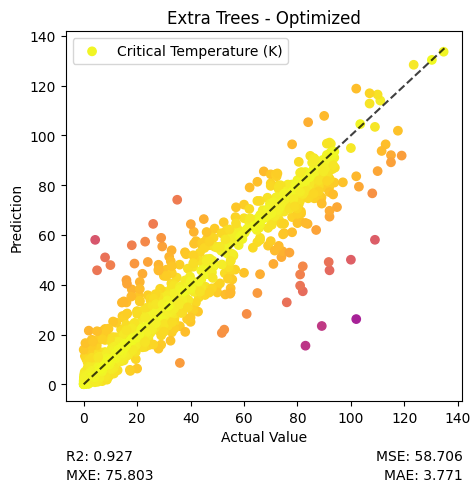
\includegraphics[height=2.25in]{images/subfigures/no_uncertainty/extra_trees_optimized.png}
   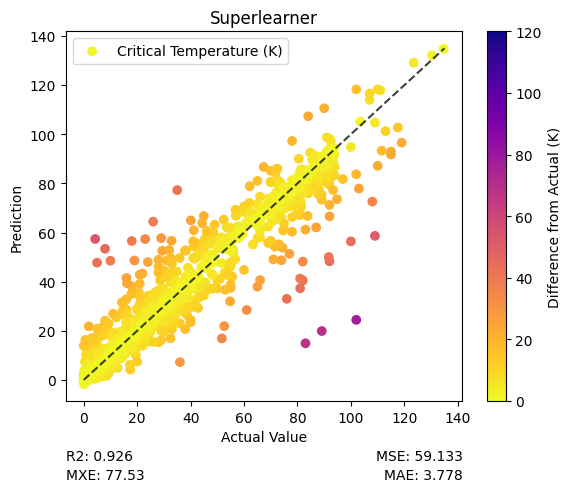
\includegraphics[height=2.25in]{images/subfigures/no_uncertainty/superlearner.png}
   \caption{Graph of optimized model predictions versus actual critical temperatures for each base model. The dotted line represents the optimal prediction for any given critical temperature.}
\end{figure*}\label{fig:results}

\begin{table*}[b]
  \resizebox{\textwidth}{!}{%
  \begin{tabular}{|lcccc|lcccc|}

  \multicolumn{5}{c}{\textbf{Unoptimized}}                                                   & \multicolumn{5}{c}{\textbf{Optimized}}                                                      \\ \hline
  \textbf{Model}                    & \textbf{R2} & \textbf{MSE} & \textbf{MAE} & \textbf{MWS} & \textbf{Model}                    & \textbf{R2} & \textbf{MSE} & \textbf{MAE} & \textbf{MWS} \\ \hline
  {Extra Trees Regression}   & 0.927       & 58.706       & 3.771        & 35.635       & {Extra Trees Regression}   & 0.927       & 58.565       & 3.792        & 35.850       \\
  {Random Forest Regression} & 0.911       & 71.209       & 4.310        & 38.504       & {Superlearner}             & 0.926       & 59.133       & 3.778        & 35.729       \\
  {KNeighbors Regression}    & 0.843       & 126.106      & 5.976        & 52.631       & {Random Forest Regression} & 0.910       & 72.112       & 4.349        & 39.254       \\
  {Decision Tree Regression} & 0.818       & 145.964      & 5.598        & 58.664       & {Decision Tree Regression} & 0.831       & 135.041      & 5.529        & 56.136       \\
  {Support Vector Machines}  & 0.710       & 232.020      & 9.026        & 64.056       & {KNeighbors Regression}    & 0.803       & 157.928      & 6.897        & 58.231       \\
  {Linear Regression}        & 0.608       & 314.499      & 13.147       & 76.753       & {Support Vector Machines}  & 0.710       & 232.020      & 9.026        & 64.056       \\
  {Elastic Net Regression}   & 0.607       & 315.162      & 13.161       & 77.033       & {Bayesian Regression}      & 0.607       & 314.711      & 13.172       & 76.994       \\
  {Bayesian Regression}      & 0.607       & 314.711      & 13.172       & 76.994       & {Elastic Net Regression}   & 0.513       & 389.897      & 14.877       & 86.375       \\ \hline
  \end{tabular}
  }
  \caption{CV scores of the models comparing optimized and base hyper-parameters.}
\end{table*}\label{tab:results}
\afterpage{\clearpage}

%move this page down if we can, after finishing draft:
\begin{figure*}[!h]
   \centering
   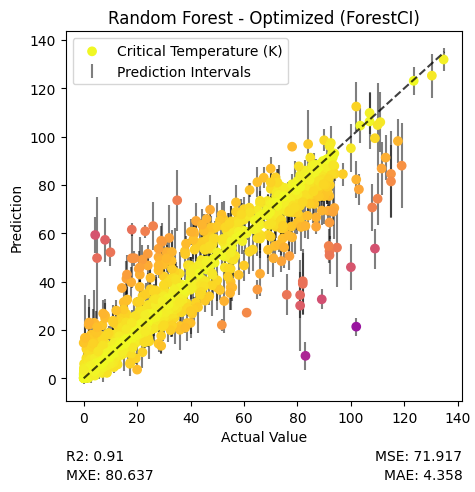
\includegraphics[height=2.25in]{images/subfigures/random_forest_optimized_forestci.png} \nolinebreak
   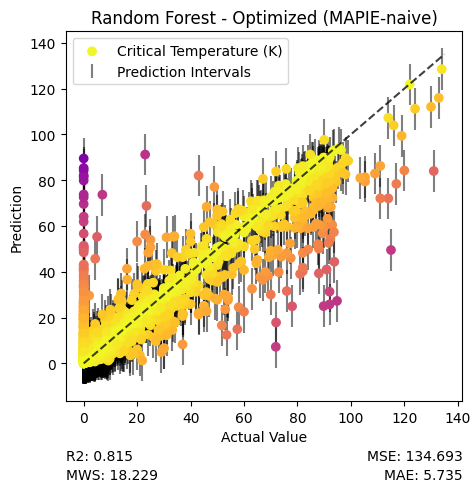
\includegraphics[height=2.25in]{images/subfigures/random_forest_optimized_mapie-naive.png} \nolinebreak
   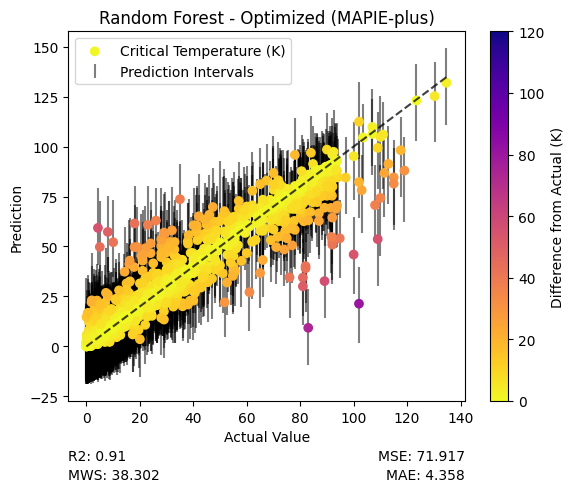
\includegraphics[height=2.25in]{images/subfigures/random_forest_optimized_mapie-plus.png}
   \caption{Comparision MAPIE methods and ForestCI uncertainty calculations for Random Forest models with plot of optimized model predictions versus actual critical temperatures. Note that all other uncertainty calculations in this paper use the MAPIE-plus method, which uses a Jackknife+ algorithm. This is the default method for MAPIE.}
\end{figure*}\label{fig:mapie-forestci}

\begin{figure*}[!h]
    \centering
    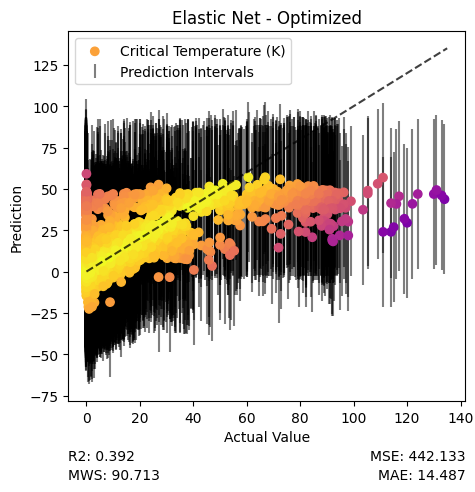
\includegraphics[height=2.25in]{images/subfigures/uncertainty/elastic_net_optimized.png}
    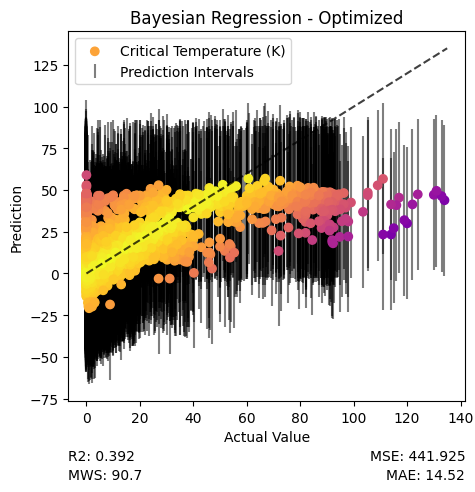
\includegraphics[height=2.25in]{images/subfigures/uncertainty/bayesian_regression_optimized.png}
    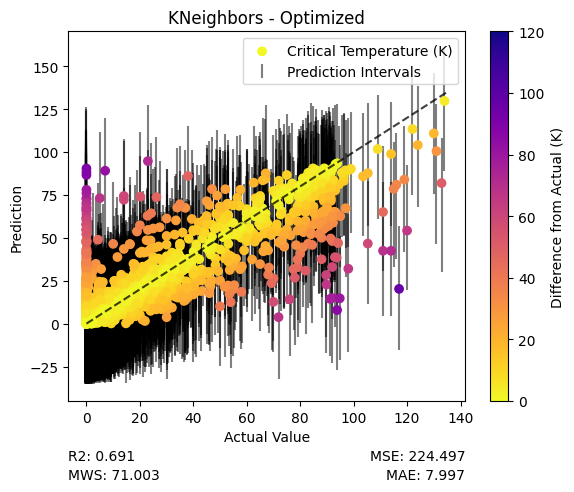
\includegraphics[height=2.25in]{images/subfigures/uncertainty/kneighbors_optimized.png}
   %  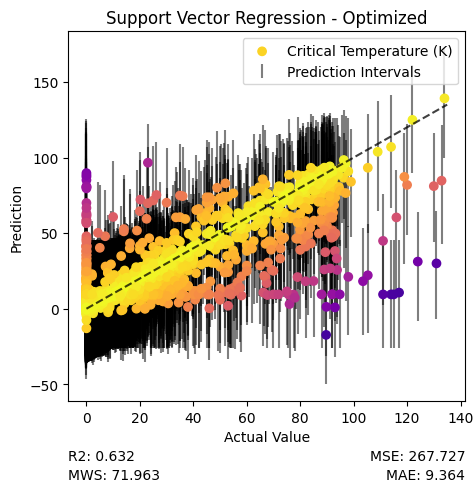
\includegraphics[height=2.25in]{images/subfigures/uncertainty/support_vector_regression_optimized.png}
   %  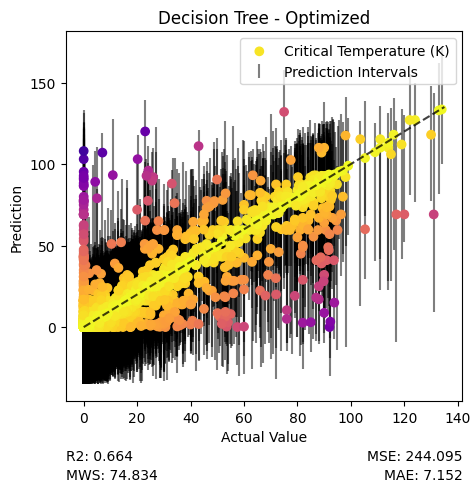
\includegraphics[height=2.25in]{images/subfigures/uncertainty/decision_tree_optimized.png}
   %  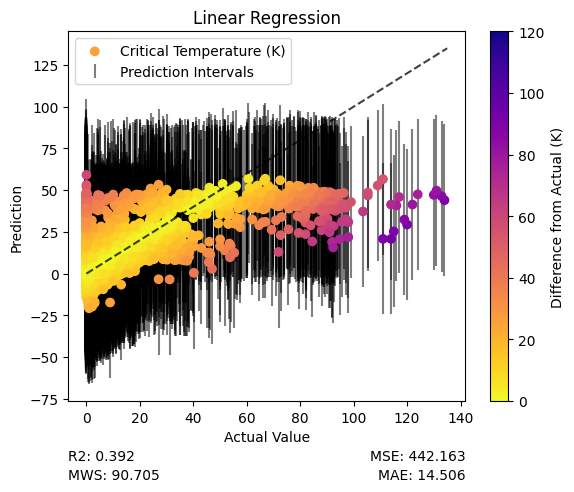
\includegraphics[height=2.25in]{images/subfigures/uncertainty/linear_regression.png}
    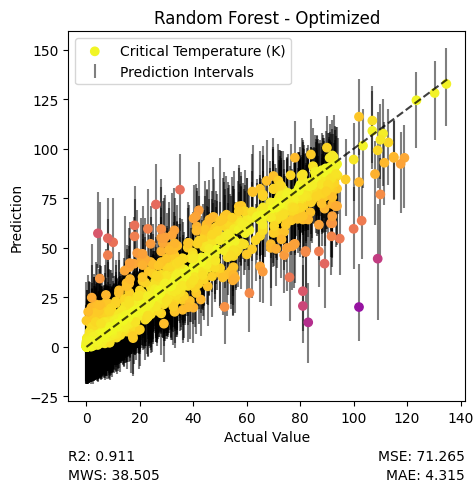
\includegraphics[height=2.25in]{images/subfigures/uncertainty/random_forest_optimized.png}
    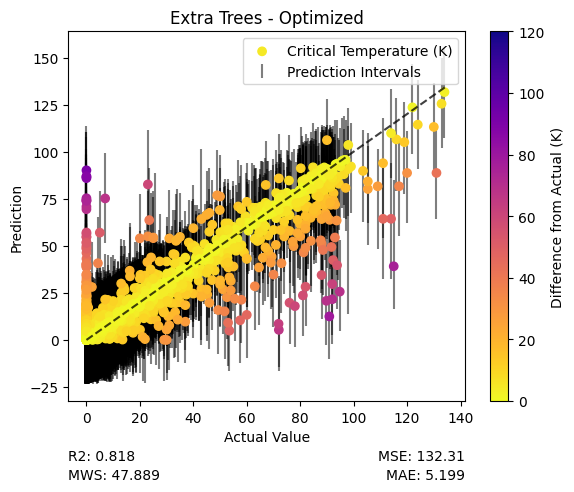
\includegraphics[height=2.25in]{images/subfigures/uncertainty/extra_trees_optimized.png}
    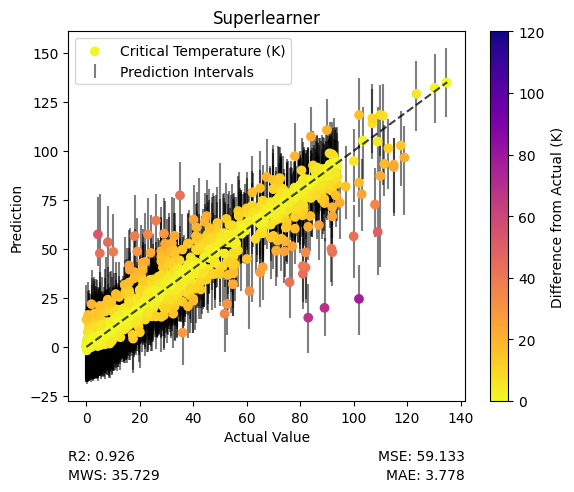
\includegraphics[height=2.25in]{images/subfigures/uncertainty/superlearner.png}
    \caption{Graph of optimized model predictions versus actual critical temperatures for selected base model with confidence intervals. Other models have similar invervals but are omitted here for brevity.}
\end{figure*}\label{fig:results-uncertainty}
\clearpage

The performance of each optimizer on selected high performance models is shown in Table~\ref{tab:optimizers}. Note that the optimal method for each model (shown in bold), was found with various methods. The Bayesian optimization was much less computationally expensive than GridSearchCV, however, and is the recommended method for large datasets.

\subsection{Optimized Models}\label{sec:optimized-models}

Our base models provided good results and the top two models, Random Forest and Extra Trees, only improved their scores marginally with optimization. Our numerical results of the optimized and optimized models are shown in Table~\ref{tab:results}.

% \begin{table}[!hb]
%    \centering
%    \resizebox{\columnwidth}{!}{%
%    \begin{tabular}{clcccc}
%    \hline
%    \multicolumn{1}{l}{}                                                                                 & \textbf{Model}                    & \multicolumn{1}{l}{\textbf{R2}} & \multicolumn{1}{l}{\textbf{MSE}} & \multicolumn{1}{l}{\textbf{MAE}} & \multicolumn{1}{l}{\textbf{MWS}} \\ \hline
%    \multirow{8}{*}{\textbf{\textbf{\rotatebox[origin=c]{90}{\parbox[c]{2cm}{\centering Unoptimized}}}}} & \textbf{Extra Trees Regression}   & 0.927                           & 58.706                           & 3.771                            & 35.635                           \\
%                                                                                                         & \textbf{Random Forest Regression} & 0.911                           & 71.209                           & 4.310                            & 38.504                           \\
%                                                                                                         & \textbf{KNeighbors Regression}    & 0.843                           & 126.106                          & 5.976                            & 52.631                           \\
%                                                                                                         & \textbf{Decision Tree Regression} & 0.818                           & 145.964                          & 5.598                            & 58.664                           \\
%                                                                                                         & \textbf{Support Vector Machines}  & 0.710                           & 232.020                          & 9.026                            & 64.056                           \\
%                                                                                                         & \textbf{Linear Regression}        & 0.608                           & 314.499                          & 13.147                           & 76.753                           \\
%                                                                                                         & \textbf{Elastic Net Regression}   & 0.607                           & 315.162                          & 13.161                           & 77.033                           \\
%                                                                                                         & \textbf{Bayesian Regression}      & 0.607                           & 314.711                          & 13.172                           & 76.994                           \\ \hline
%    \multirow{8}{*}{\textbf{\textbf{\rotatebox[origin=c]{90}{\parbox[c]{2cm}{\centering Optimized}}}}}   & \textbf{Extra Trees Regression}   & 0.927                           & 58.565                           & 3.792                            & 35.850                           \\
%                                                                                                         & \textbf{Superlearner}             & 0.926                           & 59.133                           & 3.778                            & 35.729                           \\
%                                                                                                         & \textbf{Random Forest Regression} & 0.910                           & 72.112                           & 4.349                            & 39.254                           \\
%                                                                                                         & \textbf{Decision Tree Regression} & 0.831                           & 135.041                          & 5.529                            & 56.136                           \\
%                                                                                                         & \textbf{KNeighbors Regression}    & 0.803                           & 157.928                          & 6.897                            & 58.231                           \\
%                                                                                                         & \textbf{Support Vector Machines}  & 0.710                           & 232.020                          & 9.026                            & 64.056                           \\
%                                                                                                         & \textbf{Bayesian Regression}      & 0.607                           & 314.711                          & 13.172                           & 76.994                           \\
%                                                                                                         & \textbf{Elastic Net Regression}   & 0.513                           & 389.897                          & 14.877                           & 86.375                           \\ \hline
%    \end{tabular}%
%    }
%    \caption{CV scores of the models comparing optimized and base hyperparameters.}
% \end{table}\label{tab:results}

The linear models performed a little worse, with none of these models exceeding an R2 value of 0.72, and with MAE above 8K. Additionally, uncertainty is quite high for these models, with the confidence interval widths (MWS) exceeding 60K. The decision tree and KNeighbors models perform a little better, with R2 values around 0.8 and MAE around 5K. 

Our ensemble models stole the show—the extra trees model consistently performed the best, with an R2 value of 0.927, MAE around 3.8K, and confidence intervals around 35K. Our superlearner (using optimizd Extra Trees, Random Forest, Decision Trees, and KNeighbor models) performed quite well, with a slightly smaller MAE than the Extra Trees model and marginally lower R2. Lastly, our Random Forest model had slightly worse R2 and MAE scores. These results are shown graphically in Figure~\ref{fig:results}.

As shown in Figure~\ref{fig:results}, the linear models do not make good predictions at high critical temperatures. All the linear models make very similar predictions - the ensemble methods and KNeighbors have better predictions and are less uniform.

\subsection{Comparing Uncertainty}
As discussed in Section~\ref{sec:uncertainty}, we quantified uncertainty for our predictions, mainly using MAPIE. Since our other uncertainty libraries only work for Random Forest Models, we used MAPIE to evaluate our models. We trained a Random Forest Model model with ForestCI to compare with MAPIE methods of uncertainty quantification. 

As shown in Figure~\ref{fig:mapie-forestci}, MAPIE's naive confidence interval method has very similar to the ForestCI calculations. MAPIE has other prediction methods (base and minmax) that produce somewhat similar results to the MAPIE-plus (Jackknife+) method, but since we are not using those algorithms, we chose to compare our selected MAPIE method and the ForestCI-like method to compare to ForestCI.

ForestCI and MAPIE-naive produce very similar results, with MAPIE-naive making slightly more optimistic prediction intervals. However, MAPIE-plus produces prediction intervals which intersect with the actual value much more reliably. Thus, MAPIE-plus may be a better choice for our models, regardless of ForestCI's limited scope (only Random Forest Regression models).

\subsection{Uncertainty Models}
Since MAPIE is model agnostic, we have uncertainty predictions for all our models. We discussed our chosen MAPIE numerical uncertainty metric in Section~\ref{sec:optimized-models}, but we can also represent the prediction interval graphically, showing the prediction interval for each predicted point. This is shown in Figure~\ref{fig:results-uncertainty}.

In Figure~\ref{fig:results-uncertainty}, each point has error bars that show the confidence interval. The model can be visually evaluated by seeing how many of the error bars intersect the dotted line, which represents the ideal prediction. While smaller prediction intervals are great, a model is not useful if it most predictions are not within error of the actual value. The bottom three models, ensemble models, have the smallest error bars and most prediction points have the actual value within the prediction interval. 

The linear models in Figure~\ref{fig:results-uncertainty} have unacceptablely large prediction intervals, in addition to their poor R2 and error metrics. KNeighbors is slightly better, but the uncertainty is still very high. Once again, our ensemble methods show the best metrics, with much smaller prediction intervals that still almost always include the actual value.

\subsection{Feature Selection}

\begin{figure}[!h]
   \centering
   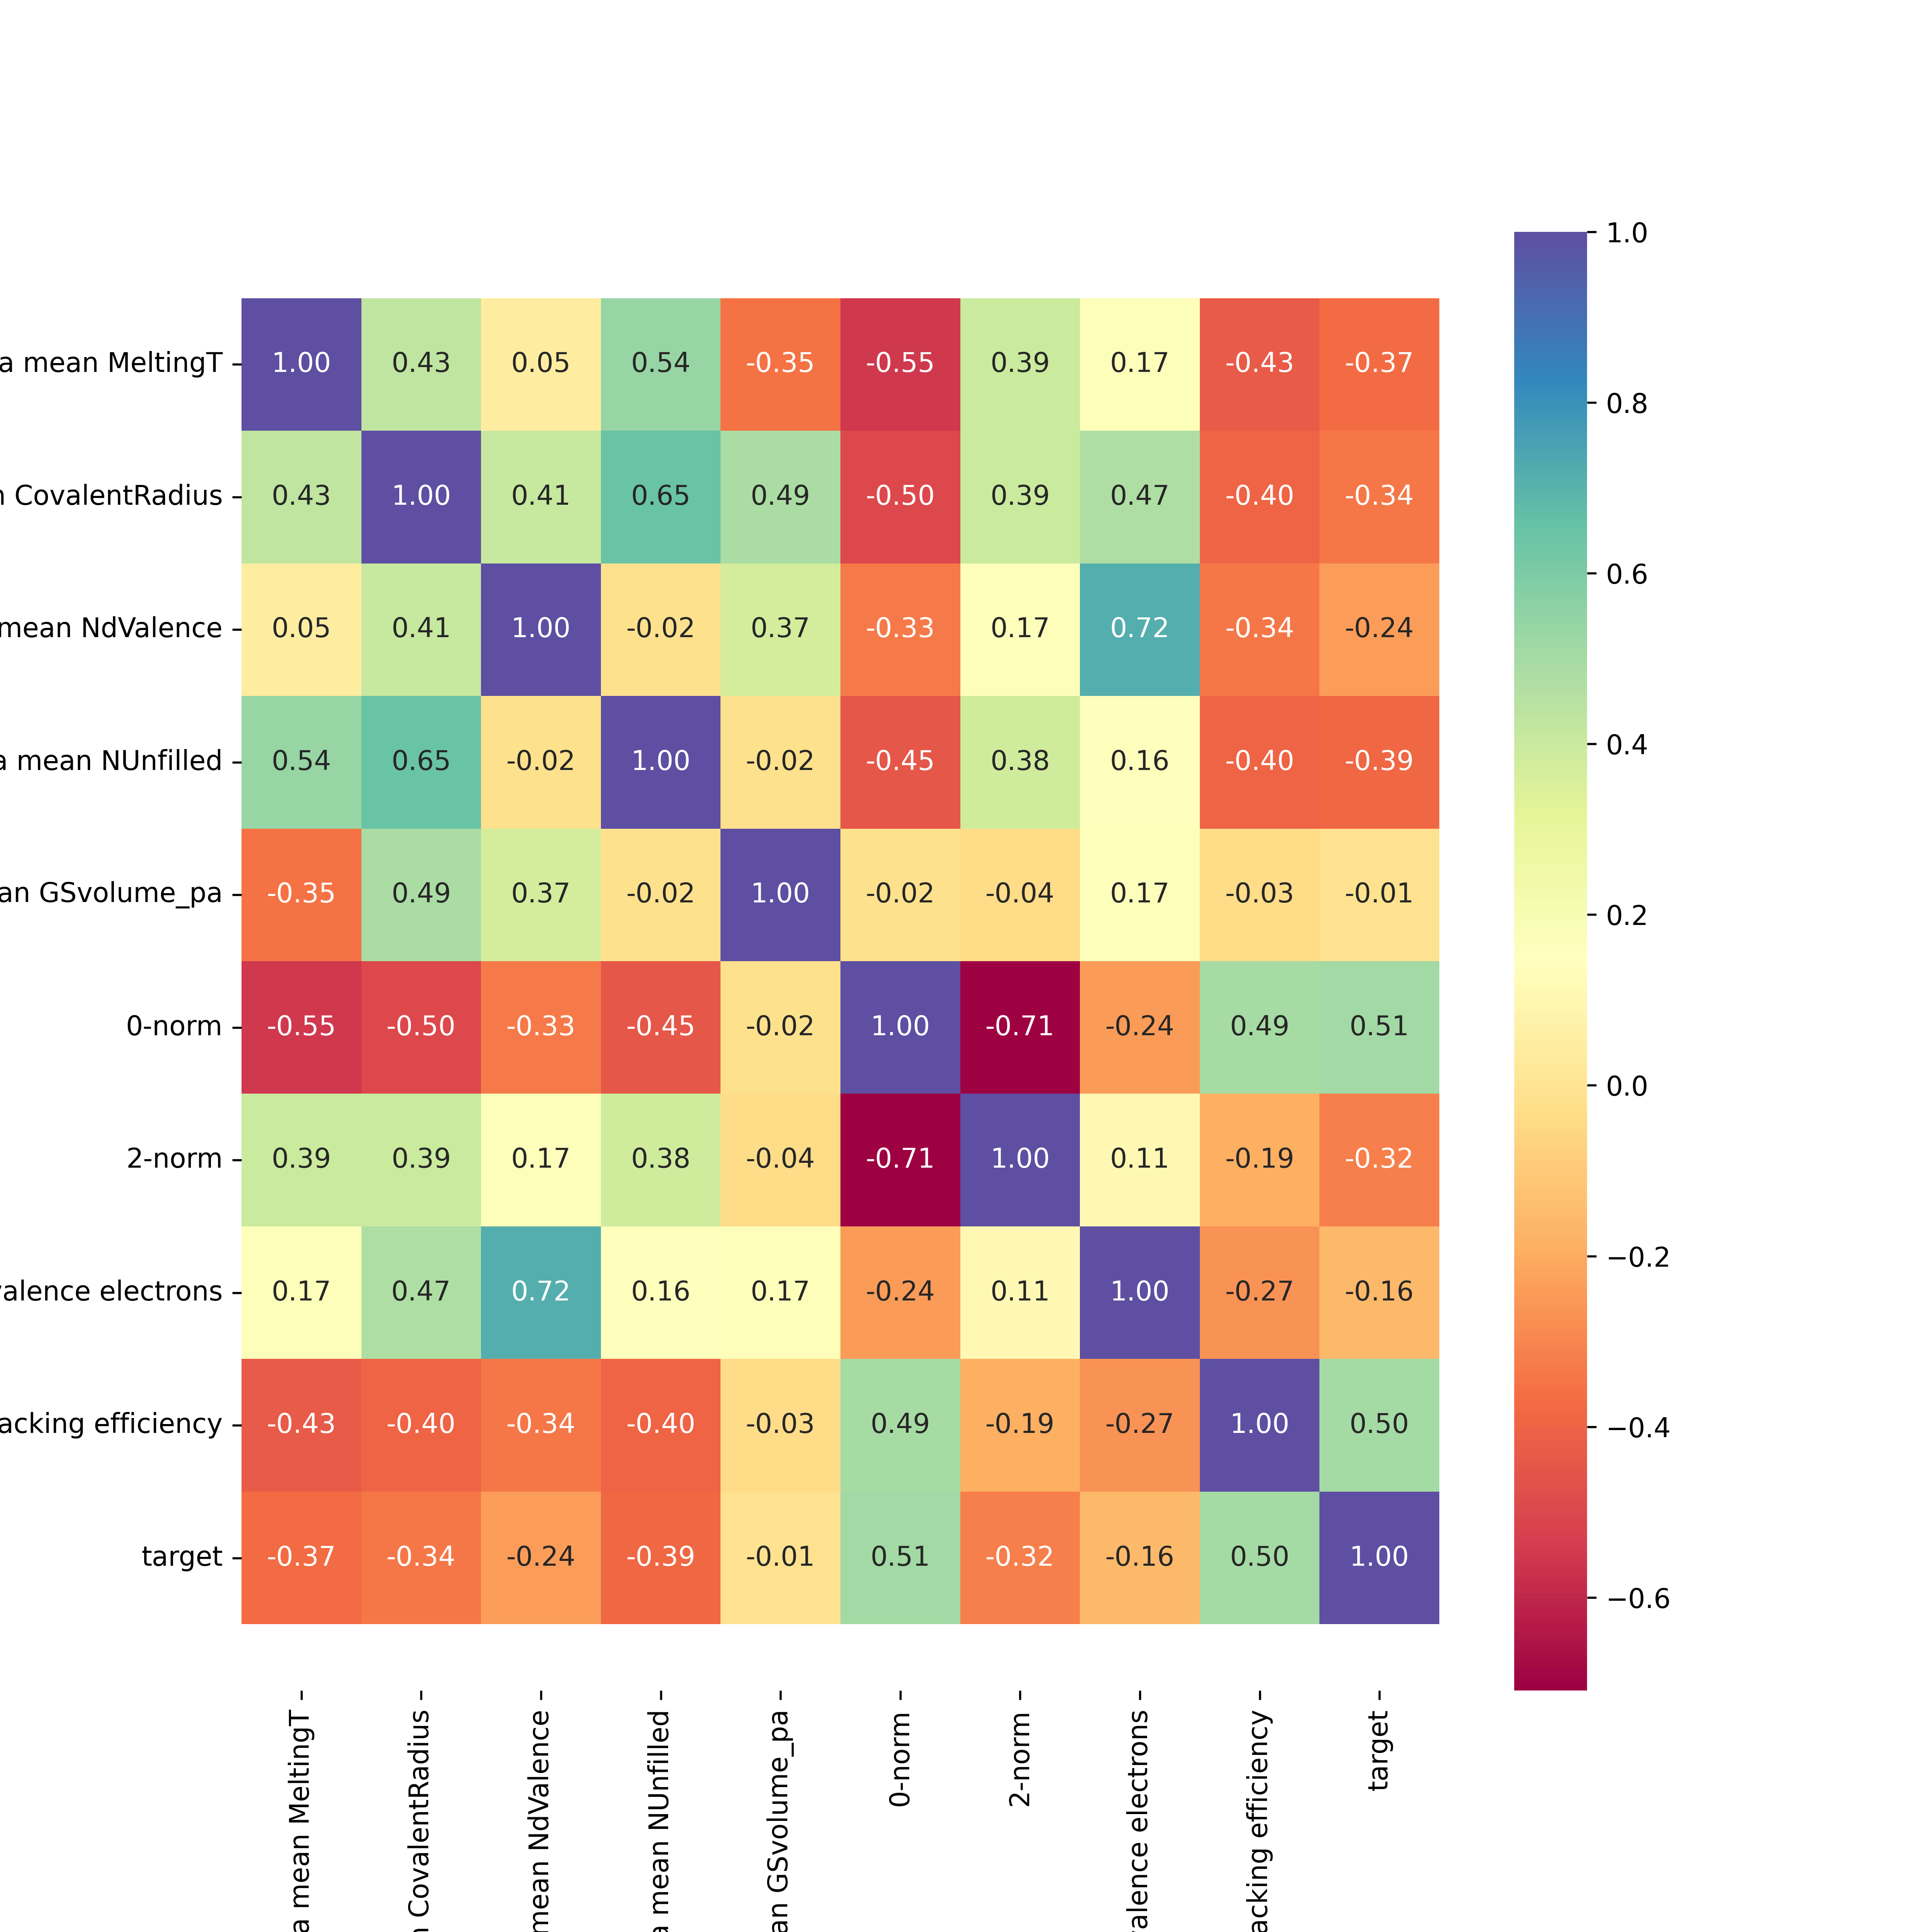
\includegraphics[width=\columnwidth]{images/feature_heatmap_eti.png}
   \caption{Heatmap of correlations between most important features for our Extra Trees model and the critical temperatures.}
\end{figure}\label{fig:feature-correlations}

\begin{figure*}[]
   \centering
   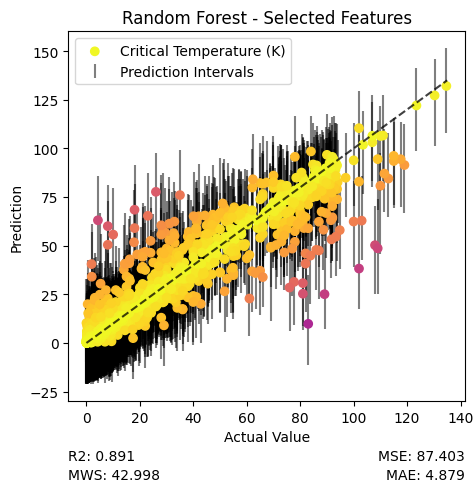
\includegraphics[height=2.25in]{images/subfigures/random_forest_selected_features.png}\nolinebreak
   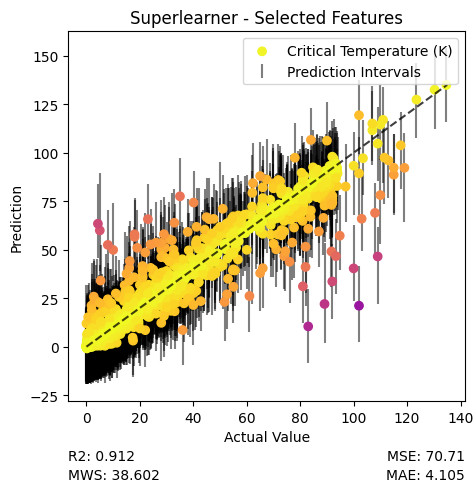
\includegraphics[height=2.25in]{images/subfigures/superlearner_selected_features.png}\nolinebreak
   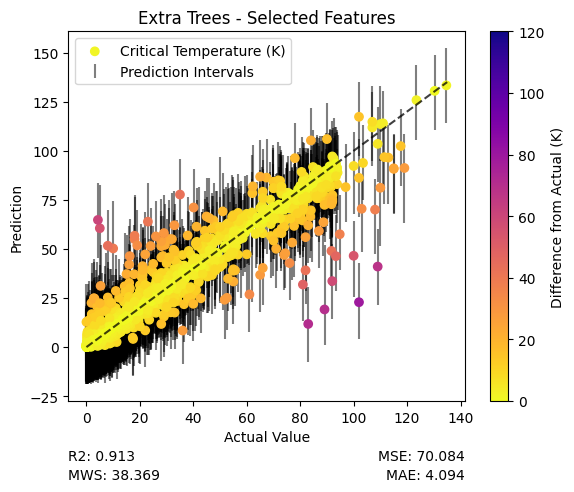
\includegraphics[height=2.25in]{images/subfigures/extra_trees_selected_features.png}
   \caption{Top three optimized models, using their top ten most important features. Note that the Superlearner model is using the Extra Trees feature importance, as the mlens model does not have a feature importance method.}
\end{figure*}\label{fig:selected-features}

\begin{figure*}[]
   \centering
   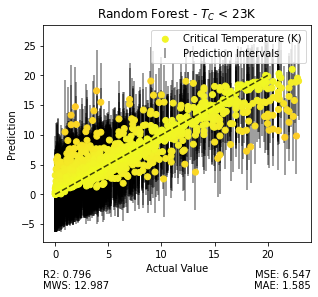
\includegraphics[height=2.5in]{images/subfigures/random_forest_t_c_<_23k.png}%\\
   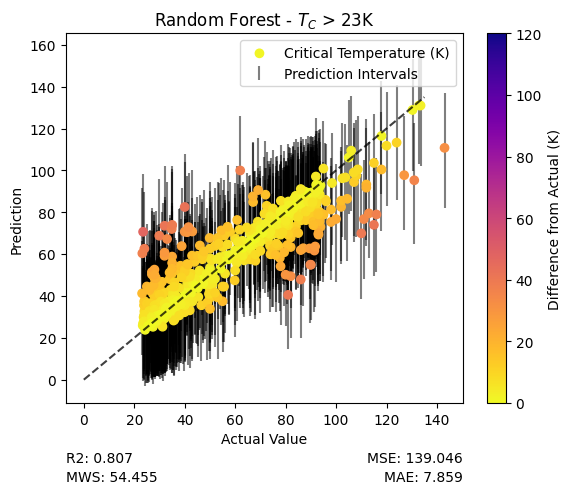
\includegraphics[height=2.5in]{images/subfigures/random_forest_t_c_>_23k.png}\\
   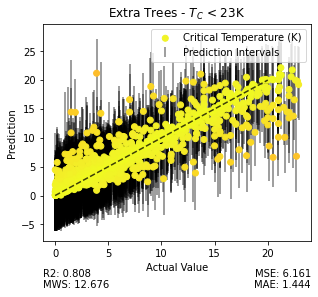
\includegraphics[height=2.5in]{images/subfigures/extra_trees_t_c_<_23k.png}
   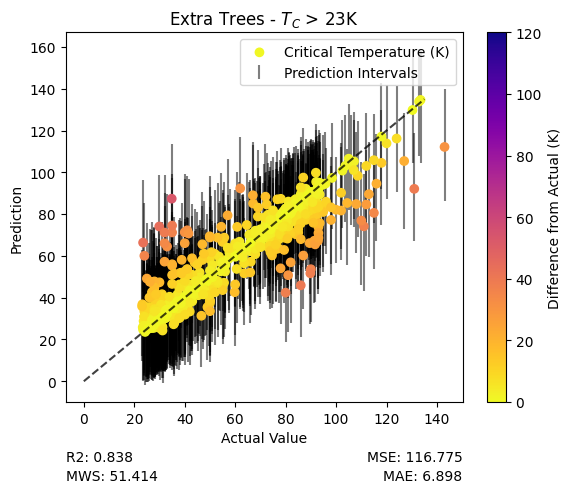
\includegraphics[height=2.5in]{images/subfigures/extra_trees_t_c_>_23k.png}
   \caption{Random Forest and Extra Trees models using temperature limited data, $T_C$ above or below 23K.}
\end{figure*}\label{fig:temp-limited}

The results shown thus far have included all features produced with matminer. We decided to perform some feature selection to reduce complexity and training time for our models. First, we used Scikit-Learn's feature importance method for our ensemble methods to find the relative importance for each model. The most important features for Random Forest and Extra Trees are shown in Table~\ref{tab:feature-importance}. Notably, Table~\ref{tab:feature-importance} shows that both models have the same top two features, with varying less important features below it.

\begin{table}[!h]
   \centering
   \resizebox{\columnwidth}{!}{%
   \begin{tabular}{|lc|}
   \hline
   \multicolumn{2}{|c|}{\textbf{Extra Trees}}                      \\ \hline
   \textbf{Feature}                          & \textbf{Importance} \\
   Mean Absolute Sim. Packing Efficiency & 15.62\%             \\
   Mean NUnfilled                            & 7.71\%              \\
   0-norm                                    & 6.67\%              \\
   Mean NfUnfilled                           & 3.25\%              \\
   Mean NdUnfilled                           & 3.25\%              \\
   Mean SpaceGroupNumber                     & 3.02\%              \\
   Mean Electronegativity                    & 2.95\%              \\
   2-norm                                    & 2.79\%              \\ \hline
   \multicolumn{2}{|c|}{\textbf{Random Forest}}                    \\ \hline
   \textbf{Feature}                          & \textbf{Importance} \\
   Mean Absolute Sim. Packing Efficiency & 32.73\%             \\
   Mean NUnfilled                            & 11.53\%             \\
   D Valence $e^-$                           & 3.80\%              \\
   0-norm                                    & 3.66\%              \\
   Mean MeltingT                             & 2.68\%              \\
   Mean GSvolume\_pa                         & 2.52\%              \\
   2-norm                                    & 2.44\%              \\
   10-norm                                   & 2.12\%              \\ \hline
   \end{tabular}%
   }
   \caption{Comparison of feature importance for Scikit-Learn ensemble models. Note that the top two features are the same for all three models.}
\end{table}\label{tab:feature-importance}


%  switch to this table if possible (horizontal, star enviroment being impossible)
% \begin{table*}[!t] 
%    \centering
%    \resizebox{\textwidth}{!}{%
%    \begin{tabular}{|lc|lc|lc}
%    \hline
%    \multicolumn{2}{|c|}{\textbf{Extra Trees}}                      & \multicolumn{2}{c|}{\textbf{Random Forest}}                     & \multicolumn{2}{c|}{\textbf{Decision Trees}}                                          \\ \hline
%    \textbf{Feature}                          & \textbf{Importance} & \textbf{Feature}                          & \textbf{Importance} & \textbf{Feature}                          & \multicolumn{1}{c|}{\textbf{Importance}} \\
%    $\lvert\mu \rvert$ Sim. Packing Efficiency\footnote{$\lvert\mu \rvert$ Sim. Packing Efficiency is the mean absolute value of the simulated packing efficiency.} & 15.62\%             & $\lvert\mu \rvert$ Sim. Packing Efficiency & 32.73\%             & $\lvert\mu \rvert$ Sim. Packing Efficiency & \multicolumn{1}{c|}{32.90\%}             \\
%    Mean NUnfilled                            & 7.71\%              & Mean NUnfilled                            & 11.53\%             & Mean NUnfilled                            & \multicolumn{1}{c|}{11.83\%}             \\
%    0-norm                                    & 6.67\%              & frac d valence electrons                            & 3.80\%              & frac d valence electrons                  & \multicolumn{1}{c|}{4.57\%}              \\
%    Mean NfUnfilled                           & 3.25\%              & 0-norm                                    & 3.66\%              & Mean NdValence                            & \multicolumn{1}{c|}{3.53\%}              \\
%    Mean NdUnfilled                           & 3.25\%              & Mean MeltingT                             & 2.68\%              & 0-norm                                    & \multicolumn{1}{c|}{3.43\%}              \\
%    Mean SpaceGroupNumber                     & 3.02\%              & Mean GSvolume\_pa                          & 2.52\%              & Mean MeltingT                             & \multicolumn{1}{c|}{3.42\%}              \\
%    Mean Electronegativity                    & 2.95\%              & 2-norm                                    & 2.44\%              & Mean CovalentRadius                       & \multicolumn{1}{c|}{2.94\%}              \\
%    2-norm                                    & 2.79\%              & 10-norm                                   & 2.12\%              & 2-norm                                    & \multicolumn{1}{c|}{2.87\%}              \\ \hline
%    \end{tabular}%
%    }
%    \caption{Comparison of feature importance for Scikit-Learn ensemble models. Note that the top two features are the same for all three models.}
% \end{table*}\label{tab:feature-importance}
Finally, we trained some models on temperature limited data, temperatures above 23K or below 23K. The models, shown in Figure~\ref{fig:temp-limited}, show the weaknesses of the models. While the high temperature model has a higher R2, the error and uncertainty scores are much worse than the low temperature model. This reflects our understanding of superconductors. We know little about unconventional temperature superconductors and have limited data on them, so our model is likely to have higher error at those points.

Next, we trained three models using only the most important features for the given model. The results are shown in Figure~\ref{fig:selected-features}. Each model has slightly worse metrics than the full model, but the decreased complexity of the model is valuable.

We also used our top model's most important features and made a correlations plot, shown in Figure~\ref{fig:feature-correlations}. A full correlation plot is available on github, but is too large for this paper.

\section{Conclusions}
\subsection{Future Work}


\begin{acknowledgments}
I would like to thank my mentor, Suchismita Sarker, for her guidance and support with this project. This work is supported by the U.S. National Science Foundation under award number NSF PHY-2150125, REU Site: Accelerator Physics and Synchrotron Radiation Science.
\end{acknowledgments}


\bibliographystyle{apsrev4-2}
\bibliography{reu-report}



\end{document}